\chapter{Siemens case}

Siemens Wind Power is among the leading windmill manufacturers in the world.
Siemens primarily do mill farms as parks, although the system handles single mills as well as entire parks.

Siemens has a need for their system to scale better and provide increased redundancy.
In the current setup (see \cref{fig:currentSiemensSetup}) the Park Monitor is a single point of failure.
Siemens has a vision of removing this component and make it into a distributed system, distributed among the windmills.

\begin{figure}
	\centering
	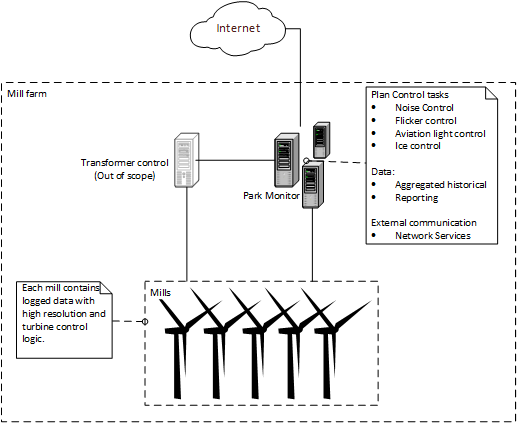
\includegraphics[width=0.8\textwidth,natwidth=610,natheight=642]{SystemOverviews.png} 
	\captionsetup{format=plain,font=footnotesize,labelfont={bf,red},labelsep=quad,singlelinecheck=no}
	\caption[Illustrates the current Siemens windmill farm setup]{
		\label{fig:currentSiemensSetup} 
		\footnotesize{%
			This figure illustrates the current Siemens windmill farm setup.
		}
	}
\end{figure}

\begin{figure}
	\centering
	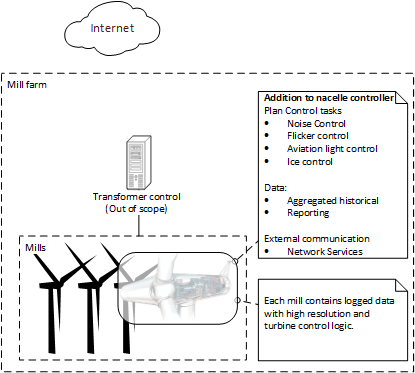
\includegraphics[width=0.8\textwidth,natwidth=610,natheight=642]{SystemOverviewsFuture.png} 
	\captionsetup{format=plain,font=footnotesize,labelfont={bf,red},labelsep=quad,singlelinecheck=no}
	\caption[Illustrates the future Siemens windmill farm setup]{
		\label{fig:futureSiemensSetup} 
		\footnotesize{%
			This figure illustrates the future Siemens windmill farm setup.
		}
	}
\end{figure}
